\newpage
\section{Model Synchronization}
\genHeader

At this point in the handbook, you have successfully created a trio of rules that can transform a \texttt{Box} with any number of \texttt{Partitions} and
\texttt{Cards} into a \texttt{Dictionary} with an unlimited number of \texttt{Entrys} (or vice versa). Your source and target models are complete, and given
that you probably won't make any further changes to your rules, your correspondence models are also complete.

Now suppose you wanted to make a minor change to one of your current instances, such as adding a single card to a partition, or removing an entry from a
dictionary? It's redundant and potentially time-consuming to run the entire transformation \emph{again}, generating an identical graph triple for a slightly
different result. Luckily, you can synchronize your models using the graph triple, only making changes in the places that actually need it! Let's begin by
implementing a forward synchronization from \texttt{Box} to \texttt{Dictionary} by adding another card to \texttt{Partition 2}.

\begin{itemize}

\item[$\blacktriangleright$] The first step is to specify your desired changes, so open \texttt{TGGmain} and complete the empty \texttt{changeSrc} method as
depicted in Fig.~\ref{eclipse:changeSrc}. 

\vspace{0.5cm}

\begin{figure}[htbp]
\begin{center}
  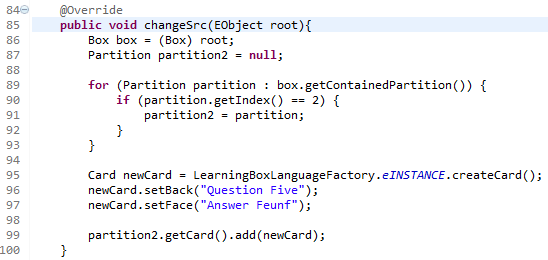
\includegraphics[width=\textwidth]{eclipse_changeSrc}
  \caption{Declaring changes to the source \texttt{Box} model}
  \label{eclipse:changeSrc}
\end{center}
\end{figure}

\vspace{0.5cm}

\item[$\blacktriangleright$] As you're completing \texttt{changeSrc}, you'll notice several error messages appear. A few additional classes need to be directly
imported from \texttt{LearningBoxLanguage}, so add the import statements in Fig.~\ref{eclipse:changeSrcImports}.

\newpage

\begin{figure}[htbp]
\begin{center}
  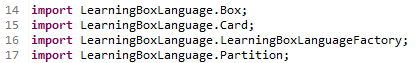
\includegraphics[width=0.8\textwidth]{eclipse_changeSrcImports}
  \caption{caption}
  \label{eclipse:changeSrcImports}
\end{center}
\end{figure}

\item[$\blacktriangleright$] It should be mentioned that you are able to implement \texttt{changeSrc} with SDMs, but here we'll just use a basic Java
implementation to avoid getting sidetracked.

\item[$\blacktriangleright$] As you can see, we begin declaring our changes in \texttt{changeSrc} by initializing the objects to be updated. The \texttt{for}
loop cycles through every \texttt{partition} in \texttt{box} until it matches to \texttt{partition2}. The \texttt{Learn\-ing\-Box\-Lang\-uage\-Fact\-ory} is then
called to create our new card, for which we then assign the \texttt{back} and \texttt{front} attributes. Finally, we add the card to the partition.
 
\item[$\blacktriangleright$] Now we have to tell \texttt{TGGMain} how to execute the change. Add a new \texttt{synchForward} method anywhere in the file, and
complete it as depicted in Fig.~\ref{eclipse:SynchForwardMethod}.

\vspace{0.5cm}

\begin{figure}[htbp]
\begin{center}
  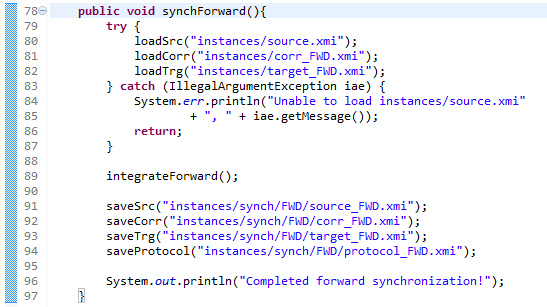
\includegraphics[width=\textwidth]{eclipse_synchForwardMethod}
  \caption{forward synchronization}
  \label{eclipse:SynchForwardMethod}
\end{center}
\end{figure}

\newpage

\item[$\blacktriangleright$] You may have noticed that this is nearly identical to the original \texttt{performForward} transformation method. The key
difference however is that we're loading every file in the triple, executing \texttt{changeSrc} via \texttt{integrateForward}, then saving the newest triple
(and protocol) in different directory. Of course, you can change this to overwrite the original files, but we have separated them in this example to
distinguish the effects of synchronization.

\item[$\blacktriangleright$] Finally, update \texttt{main} to include \texttt{synchForward()} (Fig.~\ref{eclipse:helperFWD}), and run
\texttt{TGGMain}.\footnote{If you don't comment out the previous \texttt{performForward} or \texttt{performBackward} commands, please note that the complete
TGG transformation will still run.}

\begin{figure}[htbp]
\begin{center}
  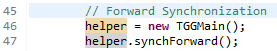
\includegraphics[width=0.5\textwidth]{eclipse_helperFWDSynch}
  \caption{comment}
  \label{eclipse:helperFWD}
\end{center}
\end{figure}

\item[$\blacktriangleright$] Navigate to ``instances/synch/FWD/'' and open \texttt{source\_FWD.xmi}. Is there now a fifth card in \texttt{parition2}? How about
a fifth \texttt{entry} in \texttt{target\_FWD} ? If your synchronization was successful, both of these should exist!

\item[$\blacktriangleright$] Compare these two new models to the original source and targets in ``instances/.'' You'll notice they don't match -- perfect! While
the synchronization started and changed these original files, the newest triple was saved in the ``FWD'' directory.

\item[$\blacktriangleright$] Let's check out what was created in \texttt{corr\_FWD.xmi}. Running the integrator on the file and proceeding as far as you can,
you'll notice that it doesn't take very long. In fact, only one thing happens! If you inspect the window, you'll be able to see that the only thing this
correspondence model shows is the creation of a single card. Because the models never had to be created from scratch, the correspondence only shows trace
information for the elements you updated.

\newpage

\item[$\blacktriangleright$] Now let's try synchronizing in the opposite direction, from Dictionary to Box. We want to remove \texttt{Entry} `One: Eins,' and
add `Six: Sechs.' Complete \texttt{changeTrg()} as shown in Fig.~\ref{eclipse:changeTrg}.

\vspace{0.5cm}

\begin{figure}[htbp]
\begin{center}
  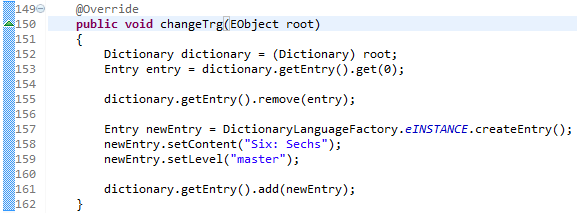
\includegraphics[width=\textwidth]{eclipse_changeTrg}
  \caption{Modifying target model}
  \label{eclipse:changeTrg}
\end{center}
\end{figure}

\item[$\blacktriangleright$] You can add the statements in Fig.~\ref{eclipse:changeTrgImports} to get rid of any errors.

\vspace{0.5cm}

\begin{figure}[htbp]
\begin{center}
  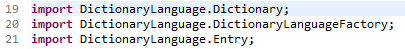
\includegraphics[width=0.8\textwidth]{eclipse_changeTrgImports}
  \caption{comment}
  \label{eclipse:changeTrgImports}
\end{center}
\end{figure}

\item[$\blacktriangleright$] Nearly identical to \texttt{synchForward}, create a new method \texttt{synchBackwards} and complete it as depicted in
Fig.~\ref{eclipse:SynchBackwardMethod}.

\begin{figure}[htbp]
\begin{center}
  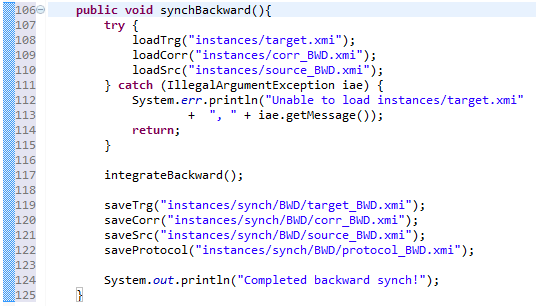
\includegraphics[width=0.9\textwidth]{eclipse_synchBackwardMethod}
  \caption{synch backwards}
  \label{eclipse:SynchBackwardMethod}
\end{center}
\end{figure}

\item[$\blacktriangleright$] Finally, re-initalize \texttt{helper} one more time to implement the synchronization function. Your final \texttt{main} method
should then resemble Fig.~\ref{eclipse:TGGSynchMain}.

\begin{figure}[htbp]
\begin{center}
  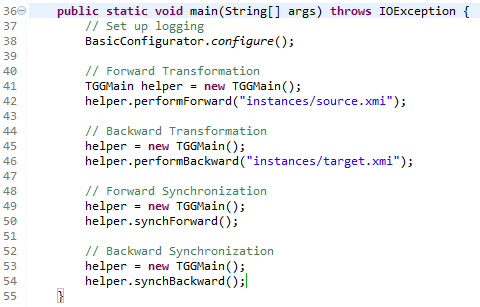
\includegraphics[width=0.9\textwidth]{eclipse_TGGSynchMain}
  \caption{Final Main method}
  \label{eclipse:TGGSynchMain}
\end{center}
\end{figure}

\item[$\blacktriangleright$] After running \texttt{TGGMain}, inspect \texttt{target\_BWD} and \texttt{source\_BWD} in ``instances/synch/BWD/.'' If your
synchronization was successful, you'll notice that you input \texttt{Dictionary} no longer has entry one, and entry six was added, reflected in
\texttt{partition0} in the output \texttt{Box}. 

\item[$\blacktriangleright$] You should also notice that there is no \texttt{Entry Four}, created in the forward synchronization. In \texttt{synchBackward}, we
specified that the synchronization should load the \emph{original} target model, not the most recent result. We encourage you to experiment with your files and
change this to create a fully streamlined process, from the original transformation to any updates by modifying the input filenames and output
directories.

\newpage

\item[$\blacktriangleright$] On a final note, try running the integrator on the newest \texttt{corr\_BWD}, and proceed as far as possible
(Fig.~\ref{eclipse:synchBwdIntegrator}). Notice how the model doesn't show the deletion of entry one? Recall that the rules of any TGG are by definition,
monotoic. The only specify the evolution or construction of the triple -- a different component of eMoflon takes care of any destructive changes. As a result,
the card essentially `disappears' from all models.

\begin{figure}[htbp]
\begin{center}
  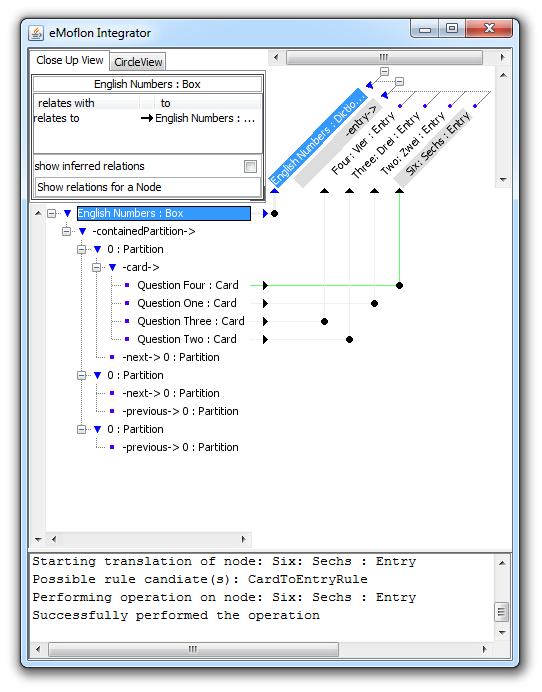
\includegraphics[width=0.9\textwidth]{eclipse_integratorCorrBWD}
  \caption{comment}
  \label{eclipse:synchBwdIntegrator}
\end{center}
\end{figure}

\end{itemize}
